\documentclass[hyperref={pdfpagelabels=false}]{beamer}
\usepackage{lmodern}
\usepackage{amsmath}
\usepackage{graphicx}
\title{Explaining and Forecasting Online Auction
Prices and Their Dynamics Using
Functional Data Analysis}   
\author{Christopher Thiemann} 
\date{January 29, 2019} 
\beamertemplatenavigationsymbolsempty
\setbeamercolor{footline}{fg=blue}
\setbeamerfont{footline}{series=\bfseries}
\usetheme{Madrid}
\usepackage{tikz}
\usetikzlibrary{shapes.geometric, arrows,chains}
\tikzset{
  startstop/.style={
    rectangle, 
    rounded corners,
    minimum width=3cm, 
    minimum height=1cm,
    align=center, 
    draw=black, 
    fill=red!30
    },
  process/.style={
    rectangle, 
    minimum width=3cm, 
    minimum height=1cm, 
    align=center, 
    draw=black, 
    fill=blue!30
    },
  decision/.style={
    rectangle, 
    minimum width=3cm, 
    minimum height=1cm, align=center, 
    draw=black, 
    fill=green!30
    },
  arrow/.style={thick,->,>=stealth},
  dec/.style={
    ellipse, 
    align=center, 
    draw=black, 
    fill=green!30
    },
}
\colorlet{beamer@blendedblue}{blue!60!green}
\setbeamertemplate{headline}
{
  \begin{beamercolorbox}[colsep=1.5pt]{middle separation line head}
  \end{beamercolorbox}
  \begin{beamercolorbox}[ht=2.5ex,dp=1.125ex,%
    leftskip=.3cm,rightskip=.3cm plus1fil]{subsection in head/foot}
    \usebeamerfont{subsection in head/foot}\insertsectionnavigationhorizontal{\textwidth}{}{}
  \end{beamercolorbox}%
  \begin{beamercolorbox}[colsep=1.5pt]{lower separation line head}
  \end{beamercolorbox}
}

\setbeamertemplate{footline}{%
    \begin{beamercolorbox}[wd=\paperwidth,ht=2.25ex,dp=1ex]{date in
            head/foot}%
        \hspace*{123ex} \insertframenumber{} / \inserttotalframenumber
    \end{beamercolorbox}}%

\AtBeginSection[]{
  \begin{frame}[plain]
  \vfill
  \centering
  \begin{beamercolorbox}[sep=8pt,center,shadow=true,rounded=true]{title}
    \usebeamerfont{title}\insertsectionhead\par%
  \end{beamercolorbox}
  \vfill
  \end{frame}
}

\let\otp\titlepage
\renewcommand{\titlepage}{\otp\addtocounter{framenumber}{-1}}

\begin{document}


\begin{frame}[plain]
\titlepage
\end{frame}


\section{Introduction}

\begin{frame}{Motivation}
    \begin{itemize}
        \item Why auctions?
        \item Why dynamic functional forecasting model?
        \begin{itemize}
            \item deal with unevenly spaced observations
            \item capture price dynamics
        \end{itemize}    
    \end{itemize}
    overall structure of the paper
    \begin{itemize}
        \item recover functional object
        \item use Functional regression to relate price evolution and velocity to auction information
        \item use results to help build the forecasting model
    \end{itemize}
\end{frame}


\begin{frame}{Data}
\begin{itemize}
    \item eBay Auctions
    \item second price sealed bid with proxy bidding
    \item 7 Day duration
    \item Microsoft Xbox and Harry Potter and the half-blood prince (N=190)
    \item Responds Variable: Bid History
\end{itemize}
\end{frame}


\begin{frame}{Bid-History}
\begin{minipage}[c]{0.65\textwidth}
\includegraphics[width=\textwidth]{bid_history.JPG}
\end{minipage}
\hfill
\begin{minipage}[c]{0.3\textwidth}
\begin{itemize}
\item[] 3 Phases
\item mild in beginning
\item sparse in the middle
\item dense at the end
\end{itemize}
\begin{itemize}
\item[] 
\item bidsniping
\item unevenly spaced observations
\end{itemize}
\end{minipage}
\end{frame}

\begin{frame}{Data}
\begin{itemize}
    \item eBay Auctions
    \item second price sealed bid with proxy bidding
    \item 7 Day duration
    \item Microsoft Xbox and Harry Potter and the half-blood prince (N=190)
    \item Responds Variable: Bid History
    \item Explanatory variables: opening bid, final price, number of bids, seller rating, bidder rating, reserve price, condition, early bidding, jump bidding
\end{itemize}
\end{frame}


\begin{frame}{Functional Regression}
\begin{itemize}
    \item use FR to explore price dynamics
    \item relate functional response variable to scalar covariates
    \item Model-type: $\mathbf{y}(t)=\mathbf{X}\beta(t)+\mathbf{\varepsilon}(t)$
    \item first: recover functional data
\end{itemize}
\end{frame}

\section{Penalized smoothing spline}
    


%\begin{frame}{Irregular spacing of bids}
%\centering
%\begin{minipage}[c]{0.5\textwidth}
%\includegraphics[width=\textwidth]{Auction1}
%\end{minipage}
%\hfill
%\begin{minipage}[c]{0.5\textwidth}
%\includegraphics[width=\textwidth]{Auction2}
%\end{minipage}
%\end{frame}

    \begin{frame}{Irregular spacing of bids}
    \centering
    \begin{minipage}[c]{0.35\textwidth}
    %\includegraphics[width=\textwidth]{log_int.pdf}
    \includegraphics[width=\textwidth]{Auction2.png}
    \includegraphics[width=\textwidth]{bid_history}
    \end{minipage}
    %\hfill
    \begin{minipage}[c]{0.5\textwidth}
    \begin{itemize}
    \item log bids
    \item linearly interpolate
    \item sample from $t=t_1,...,t_n$
    \item[] 
    \item[] 
    \end{itemize}
    \begin{align*}
    \Rightarrow \mathbf{y}^{(j)}=(y_1^{(j)},...,y_n^{(j)}) \\ j=1,...,N
    \end{align*}
    \end{minipage} 
    \end{frame}
    
    \begin{frame}{Penalized smoothing spline}
    Motivation 
    \begin{align*} 
    y_i&=x(t_i)+\varepsilon_i \\ x(t)&=\sum_{k=1}^Kc_k\phi_k(t)=\mathbf{c'}\boldsymbol\phi(t) \\ 
    SMSSE(\mathbf{y}|\mathbf{c})&=\sum_{i=1}^n[y_i-\sum_{k=1}^Kc_k\phi_k(t_i)]^2
    \end{align*}
    
    measure for variability
    \begin{align*}
    PEN_m(x)&=\int[D^mx(s)]^2ds
    \end{align*}
    \end{frame} %lambda controls bias variance tradeoff
    
    
    \begin{frame}{Penalized smoothing spline} %x twice differntiable anochmal pennse aber mit x     und poen eingesetzt von oben dadrunter
    \begin{align*}
    PENNSSE^{m}_{\lambda}(x|\mathbf{y})=\sum_{i=1}^n (y_i^{}-x^{}(t_i))^2+\lambda \int[D^mx(s)]^2ds
    \end{align*}
    \begin{itemize}
    \item[] $\lambda$ smoothing parameter
    \item[] $\lambda \rightarrow \infty \ \Rightarrow $ Linear Regression
    \item[] $\lambda = 0 \ \ \  \Rightarrow$ interpolant 
    \end{itemize}
    \begin{itemize}
    \item[] $\hat{\mathbf{c}}=(\boldsymbol\Phi'\boldsymbol\Phi+\lambda\mathbf{R})^{-1}\boldsymbol\Phi' \mathbf{y}\ \ \ \ \ \text{with} \ \  \ \ \mathbf{R}=\int D^m \phi(t) D^m \phi '(t)dt$
    \end{itemize}
    \end{frame}


    %\begin{frame}{Penalized smoothing spline - general old }
    %\begin{align*}
    %\mathbf{y}^{(j)}=(y_1^{(j)},...,y_n^{(j)}) \ \ \ \ \ \     j=1,...,N 
    %\end{align*}
    % 
    %
    %truncated polynomial spline
    %\begin{align*}
    %x(t)=\beta_0+\beta_2t+\beta_2t^2+...+\sum_{l=q}^L \beta_{pl}(t-\tau_l)^p_+ \\ %+ funktion einfügen
    %\end{align*}
    %penalized smoothing spline
    %\begin{align*}
    %PENN^{(j)}_{\lambda,m}=\sum_{i=1}^n (y_i^{(j)}-x^{(j)}(t_i))^2+\lambda PEN^{(j)}_m \int_{t_1}^{t_n}D^mx(s)^2     ds %wie bestimmt man lambda und m und knots?
    %\end{align*}
    %\end{frame}
    
    
    \begin{frame}{Penalized smoothing spline}
    \begin{align*}
    PENNSSE^{m}_{\lambda}(x|\mathbf{y})=\sum_{i=1}^n (y_i^{}-x^{}(t_i))^2+\lambda \int[D^mx(s)]^2ds
    \end{align*}
    \begin{itemize}
    \item $x(t)=\beta_0+\beta_2t+\beta_2t^2+...+\sum_{l=q}^L \beta_{pl}(t-\tau_l)^p_+$
    \item $m = 5 \Rightarrow \int_{}^{}D^5x(s)^2 ds$ %lambda begrpnden knots begründen usw.
    \item $\Gamma=\{0, 1, 2, 3, 4, 5, 6, 6.25, 6.5, 6.75, 6.8125, 6.875, 6.9375, 7\}$
    \item $\lambda$ is chosen "by visual inspection of the resulting functional
    objects."
    \end{itemize}
    
    \end{frame}
    
    
    \begin{frame}{Price dynamics}
    \center
    \includegraphics[width=1\textwidth]{smooth_velocity}
    \end{frame}
    
%\section{Motivating dynamics}    
\begin{frame}{Motivating Dynamics}
\center
\includegraphics[width=0.8\textwidth]{phase_plane}
\end{frame}

%\begin{frame}{conditional PPP}
%\center
%\includegraphics[width=1\textwidth]{phase_reserve}
%\end{frame}
%
%\begin{frame}{Differential Equation Model}
%$y_i \ i = 1,...,N$ functional objects \\
%$D^my_i$ m'th derivative of $y_i$
%\begin{equation}
%L=\omega_0I+\omega_1D+...+\omega_{m-1}D^{m-1}+D^m \nonumber 
%\end{equation}
%$Ly_i=0$
%
%\begin{align*}
%D^my_i=-\omega_0-\omega_1Dy_i-...-\omega_{m-1}D^{m-1}y_i  \\
%Ly_i=f_i 
%\end{align*}
%$Ly=0$
%\end{frame}

%\begin{frame}
%\begin{equation}
%SSE_{PDA}(L)=\sum_{i=1}^N\int[Ly_i(t)]^2dt
%\end{equation}
%\end{frame}

    
\section{Functional Regrssion}
    


    \begin{frame}{Functional Regression Model}
    Notation
    \begin{align*}
    \mathbf{y}(t) &= [y_1(t),...,y_N(t)] \\ \mathbf{x}_i&=[x_{i1},...,x_{iN}] \\ \mathbf{X} &= [x_1',...,x_p'] \\\mathbf{X}(t)&=\mathbf{X}  
    \end{align*}
    Model
    \begin{align*}
    \mathbf{y}(t)=\mathbf{X}\beta(t)+\boldsymbol\varepsilon(t)     
    \end{align*}
    Objective
    \begin{align*}
    IMSSE(\boldsymbol{\beta})=\int[\mathbf{y}(t)-\mathbf{X}\boldsymbol\beta(t)]'[\mathbf{y}(t)-    \mathbf{X}\boldsymbol\beta(t)]dt
    \end{align*}
    \end{frame}

\begin{frame}{Estimating the model}
\begin{itemize}
\item different approaches
\item fix a grid $t=t_1,...t_G$
\item for a fixed grid point, apply least squares
\item obtain estimates $\hat{\beta}(t_1),...,\hat{\beta}(t_G)$ 
\item smooth estimates to get functional estimate $\mathbf{\hat{\pmb{\beta}}}(t)$ 
\item repeat for $\mathbf{y}'(t)$
\item[]
\end{itemize}
\begin{equation}
IMSSE(\boldsymbol{\beta})=\int[\mathbf{y}'(t)-\mathbf{X}\boldsymbol\beta(t)]'[\mathbf{y}'(t)-    \mathbf{X}\boldsymbol\beta(t)]dt \nonumber
\end{equation}
\end{frame}

\begin{frame}{Estimated parameter curves for price evolution}
\center
\includegraphics[width=0.65\textwidth]{price_evolution}
\end{frame}


\begin{frame}{Estimated parameter curves for price velocity}
\center
\includegraphics[width=0.65\textwidth]{price_velocity}
\end{frame} 


\section{Dynamic Forecasting Model}

\begin{frame}{Dynamic forcasting model}
Four components
\begin{itemize}
    \item static predictor variables
    \item time-varying predictor variables
    \item price dynamics
    \item price lags
\end{itemize}    
\end{frame}

\begin{frame}{The model}
\begin{equation}
y(t|t-1)=\alpha+\sum_{i=1}^{Q}\beta_ix_i(t)+\sum_{j=1}^J\gamma_jD^{(j)}y(t|t-1)+\sum_{l=1}^L\eta_ly(t-l|t-l-1) \nonumber
\end{equation}
\newline \\
\begin{itemize}
    \item $x_1,...x_Q$ is the set of static and time variying predictors
    \item $D^{(j)}y(t|t-1)$ is the jth derivative
    \item $y(t-l|t-l-1)$ price lags
\end{itemize}
\end{frame}

\begin{frame}{h-step-ahead prediction}
\small
\begin{equation}
\tilde{y}(T+h|T)=\hat{\alpha}+\sum_{i=1}^{Q}\hat{\beta}_ix_i(T+h|T)+\sum_{j=1}^J\hat{\gamma}_j\tilde{D}^{(j)}y(T+h|T)+\sum_{l=1}^L\hat{\eta}_l\tilde{y}(T+h-l|T) \nonumber
\end{equation}
\normalsize
\newline
Two challenges
\begin{itemize}
    \item $\tilde{D}^{(j)}y(T+h|T)$ is not known
    \item static predictors in $x_i$ do not change over time
\end{itemize}
\end{frame}

\begin{frame}{forecasting price dynamics}
They model $D^{(j)}y(t|t-1)$ as a polynomial in $t$ with AR(R) residuals
\begin{align}
D^{(j)}y(t|t-1) =\sum_{k=0}^Ka_kt^k+\sum_{i=1}^Pb_ix_i(t)+u(t) \ \ \ t=1,...,T \nonumber \\ \nonumber \\ u(t)=\sum_{i=1}^R\phi_i u(t-i)+\epsilon(t) \ \ \ \ \epsilon(t) \sim \text{iidN}(0,\sigma^2) \nonumber
\end{align} 
\end{frame}

\begin{frame}{forcasting price dynamics}
\begin{itemize}
    \item get estimates for all $a_k$, $b_i$ and $u(t)$
    \item use estimated residuals to estimate all $\phi_i$
    \item estimate next resdidual with \begin{equation}  \tilde{u}(T+1|T)=\sum_{i=1}^R\tilde{\phi}_iu(T-i+1) \nonumber \end{equation}
    \item lastly estimate the price derivative \begin{equation} D^{(j)}\tilde{y}(T+1|T) =\sum_{k=0}^K\hat{a}_k(T+1)^k+\sum_{i=1}^P\hat{b}_ix_i(T+1|T)+\tilde{u}(T+1|T) \nonumber \end{equation}
\end{itemize}    
\end{frame}

\begin{frame}{integrating static auction infromation}%opening bid has an influence on price but this influence vanishes over time
\begin{itemize}
    \item problem $y(t)=\alpha +\beta x$
    \item OLS of $\alpha$ and $\beta$ confounded
    \item problem uncommon in time series analysis
    \item opening bid
    \item discounting
    \item $\tilde{x}(t)=x\tilde{\beta}(t)$
\end{itemize}
\end{frame}

\begin{frame}{Algorithm Outline}
\centering
\small
%\resizebox{!}{.8\textheight}{% if required
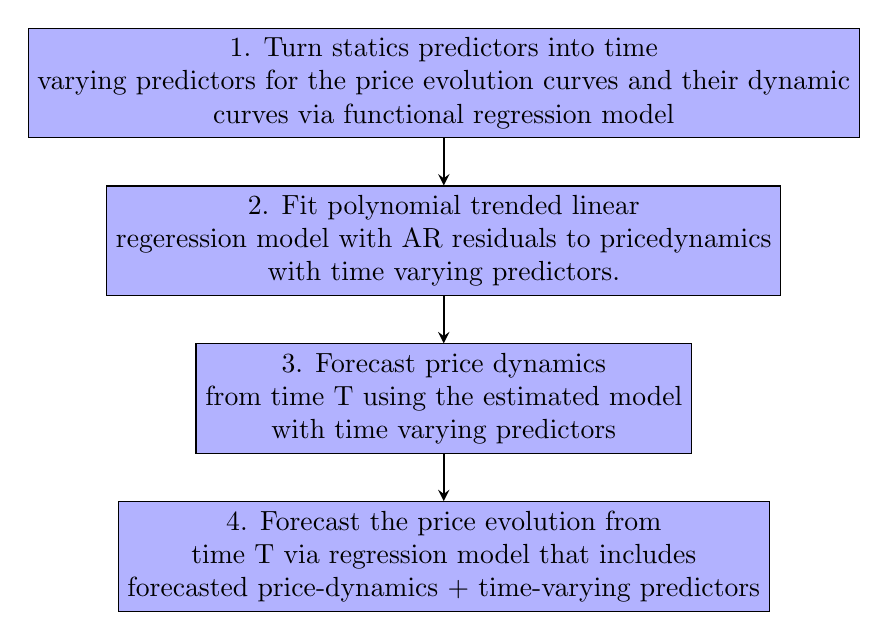
\begin{tikzpicture}[
  start chain=going below,
  every join/.style={arrow},
  node distance=0.6cm
  ]
\node (start) [process,on chain,join] {1. Turn statics predictors into time \\ varying predictors for the price evolution curves and their dynamic \\ curves via functional regression model};
\node (in1) [process,on chain] {2. Fit polynomial trended linear \\ regeression model with AR residuals to pricedynamics \\ with time varying predictors.};
\node (out1) [process,on chain,join] {3. Forecast price dynamics  \\ from time T using the estimated model \\ with time varying predictors};
\node (out2) [process,on chain,join] {4. Forecast the price evolution from \\ time T via regression model that includes  \\ forecasted price-dynamics + time-varying predictors};
\draw[arrow] (start) -- node[left] {} (in1);
\end{tikzpicture}%
%}
\end{frame}

\begin{frame}{Conclusion}
functional setup
\begin{itemize}
\item dynamic forcasting of ongoing auction
\item deals with unevenly spaced data
\item forcasting with information about derivatives
\item forcast with static and time varying variables
\end{itemize}

extension
\begin{itemize}
\item auctions of different lenght
\item incorporate concurency component
\item exact role of price dynamics not clear
\item functional differential eqquation models $\rightarrow$ principle differential analysis
\end{itemize}
\end{frame}

%\begin{frame}{Outlook}
%\begin{itemize}
%\item Motivate dynamics via Phase Plane Plots
%\item Differential Equation Model
%\item Principle Differential Analysis
%\end{itemize}
%\end{frame}

\end{document}